%%%%%%%%%%%%%%%%%%%%%%%%%%%%%%%%%%%%%%%%%
% Short Sectioned Assignment
% LaTeX Template
% Version 1.0 (5/5/12)
%
% This template has been downloaded from:
% http://www.LaTeXTemplates.com
%
% Original author:
% Frits Wenneker (http://www.howtotex.com)
%
% License:
% CC BY-NC-SA 3.0 (http://creativecommons.org/licenses/by-nc-sa/3.0/)
%
%%%%%%%%%%%%%%%%%%%%%%%%%%%%%%%%%%%%%%%%%

%----------------------------------------------------------------------------------------
%	PACKAGES AND OTHER DOCUMENT CONFIGURATIONS
%----------------------------------------------------------------------------------------

\documentclass[paper=a4, fontsize=12pt]{scrartcl} % A4 paper and 11pt font size

\usepackage[T1]{fontenc} % Use 8-bit encoding that has 256 glyphs
\usepackage{fourier} % Use the Adobe Utopia font for the document - comment this line to return to the LaTeX default
\usepackage[english]{babel} % English language/hyphenation
\usepackage{amsmath,amsfonts,amsthm} % Math packages

\usepackage{graphicx}
\usepackage{extarrows}
\usepackage{amssymb}

\usepackage{lipsum} % Used for inserting dummy 'Lorem ipsum' text into the template

\usepackage{sectsty} % Allows customizing section commands
\allsectionsfont{\centering \normalfont\scshape} % Make all sections centered, the default font and small caps

\usepackage{fancyhdr} % Custom headers and footers
\pagestyle{fancyplain} % Makes all pages in the document conform to the custom headers and footers
\fancyhead{} % No page header - if you want one, create it in the same way as the footers below
\fancyfoot[L]{} % Empty left footer
\fancyfoot[C]{} % Empty center footer
\fancyfoot[R]{\thepage} % Page numbering for right footer
\renewcommand{\headrulewidth}{0pt} % Remove header underlines
\renewcommand{\footrulewidth}{0pt} % Remove footer underlines
\setlength{\headheight}{13.6pt} % Customize the height of the header

\numberwithin{equation}{section} % Number equations within sections (i.e. 1.1, 1.2, 2.1, 2.2 instead of 1, 2, 3, 4)
\numberwithin{figure}{section} % Number figures within sections (i.e. 1.1, 1.2, 2.1, 2.2 instead of 1, 2, 3, 4)
\numberwithin{table}{section} % Number tables within sections (i.e. 1.1, 1.2, 2.1, 2.2 instead of 1, 2, 3, 4)

\setlength\parindent{0pt} % Removes all indentation from paragraphs - comment this line for an assignment with lots of text

%----------------------------------------------------------------------------------------
%	TITLE SECTION
%----------------------------------------------------------------------------------------

\newcommand{\horrule}[1]{\rule{\linewidth}{#1}} % Create horizontal rule command with 1 argument of height

\title{	
\normalfont \normalsize 
\textsc{National Sun Yat-sen University, Department of Mathematics} \\ [25pt] % Your university, school and/or department name(s)
\horrule{0.5pt} \\[0.4cm] % Thin top horizontal rule
\huge Reliability Analysis Assignment 3 \\(personal)\\ % The assignment title
\horrule{2pt} \\[0.5cm] % Thick bottom horizontal rule
}

\author{Kuan-I Chung} % Your name

\date{\normalsize 2017.04.06} % Today's date or a custom date

\begin{document}

\maketitle % Print the title

%----------------------------------------------------------------------------------------
%	3.4
%----------------------------------------------------------------------------------------
3.4
		\begin{table}[h]
			\begin{center}
			\begin{tabular}{ccrrrrrrr}
				$i$  	& 	$t_i$ 	&  	$\widehat{F}(t_i)$	&  $\widehat{F}_{(3.7)}(t_i)$ & 
				$\widehat{se}_{\widehat{F}(t_i)}$ & $C.I._L$ & $C.I._U$ & $Logit\ C.I._L$ & $Logit\ C.I._U$  \\ \hline
				1 & 33 &0.0077 &0.0077 &0.0077 &$-0.0049$ &0.0203   &0.0015   &0.0388\\
				2 & 46 &0.0154 &0.0154 &0.0108 &$-0.0024$ &0.0331   &0.0048   &0.0480\\
				3 & 50 &0.0231 &0.0231 &0.0132  &0.0014 &0.0447   &0.0090   &0.0582\\
				4 & 59 &0.0308 &0.0308 &0.0151  &0.0059 &0.0557   &0.0136   &0.0682\\
				5 & 62 &0.0385 &0.0385 &0.0169  &0.0107 &0.0662   &0.0185   &0.0781\\
				6 & 71 &0.0462 &0.0462 &0.0184  &0.0159 &0.0764   &0.0238   &0.0878\\
				7 & 74 &0.0538 &0.0538 &0.0198  &0.0213 &0.0864   &0.0292   &0.0973\\
				8 & 75 &0.0615 &0.0615 &0.0211  &0.0269 &0.0962   &0.0347   &0.1068\\
				9 & 78 &0.0769 &0.0769 &0.0234  &0.0385 &0.1154   &0.0463   &0.1253
			\end{tabular}
			\end{center}
		\end{table}

\begin{itemize}
	
	\item[(a)]{
		The answer is shown above.
	}
	
	\item[(b)]{
		The answer is shown above. Some of the lower bounds of the original confidence intervals is less than 0, and it is unreasonable. Thus, we provides a logit-transformed confidence intervals, and the two methods are shown in the following figure. We could noticed that the logit-transformed confidence band is wider but more reasonable than the original one. \\
	\newpage	
		\begin{figure}[h]
			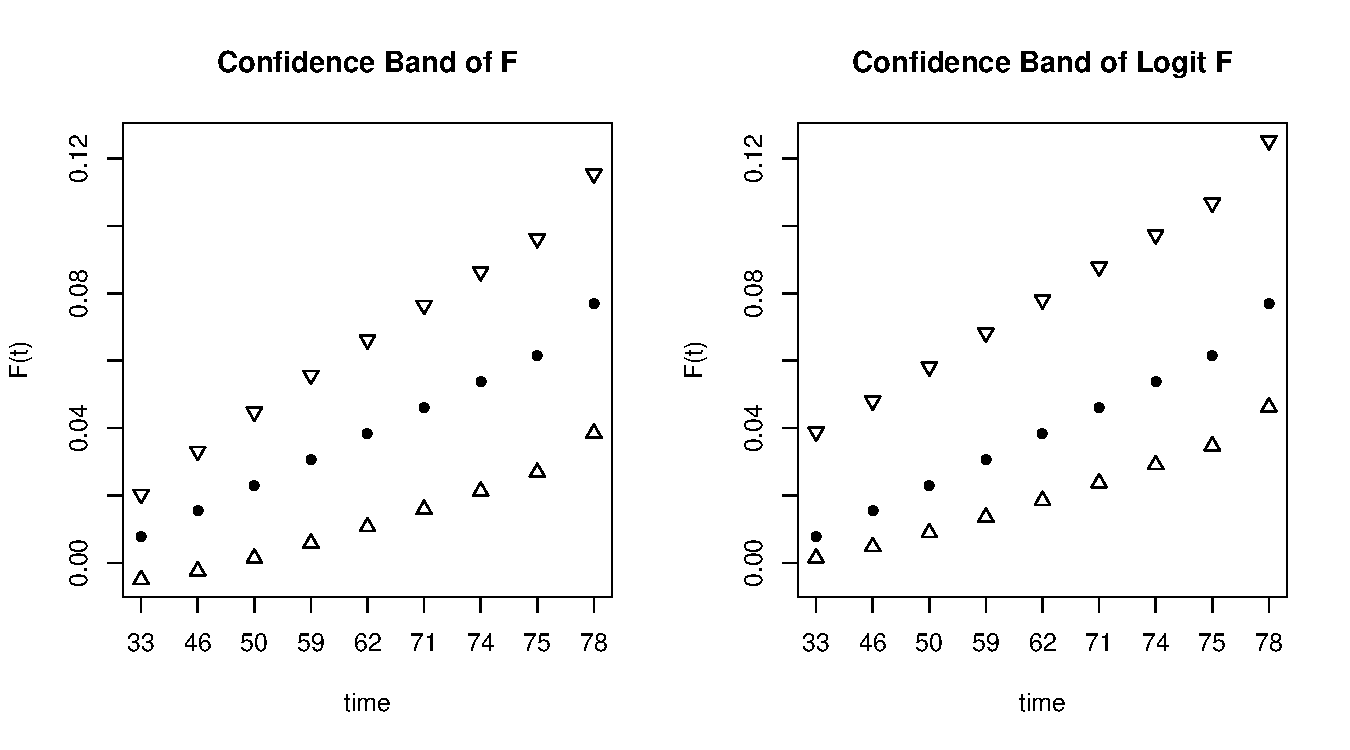
\includegraphics[width = 6 in]{3_4_b.pdf}
		\end{figure}
	}

	\item[(c)]{
		The answer is shown above. In the first three failures, the two methods have the same estimate.
	}
	
	\item[(d)]{
		The experimenter might not monitor failure occurring throughout the experiment. Also, the experiment lasted only a little time. These made us unable to predict the failure rate after 78 thousand cycles.
	}
	
	\item[(e)]{
		That would be not general enough. 
	}
	
	\item[(f)]{
		If we know the order of the starting time of the each links, than we will be able to consider the censoring effect. An that would help us predict the failure rates more precisely.
	}
\end{itemize}



%----------------------------------------------------------------------------------------
%	3.8
%----------------------------------------------------------------------------------------
3.8

\begin{align*}
				& 	L\left(F(t_i)\right) =  {n \choose \sum_{j = 1}^i d_j} \left(F(t_i)\right)^{\sum_{j = 1}^i d_j}\left(1-F(t_i)\right)^{n-\sum_{j = 1}^i d_j} \\
	\Rightarrow\ \ \ 	&	logL\left(F(t_i)\right) =  log{n \choose \sum_{j = 1}^i d_j}  + \left( \sum_{j = 1}^i d_j \right) logF(t_i) +  \left( n - \sum_{j = 1}^i d_j \right) log\left(1- F(t_i) \right)\\
	\text{Let}\ \ \ 	& \frac{\partial logL\left(F(t_i)\right)}{ \partial F(t_i)} = \frac{\sum_{j = 1}^i d_j }{F(t_i)} + \frac{n-\sum_{j = 1}^i d_j }{1-F(t_i)} = 0\ \ \ \ 
	\Rightarrow\ \ \ 		F(t_i) = \frac{\sum_{j = 1}^i d_j }{n}\\
	\because\ \ \ 	&	\left. \frac{\partial^2 logL\left(F(t_i)\right)}{ \partial F(t_i)^2} \right |_{F(t_i) = \frac{\sum_{j = 1}^i d_j }{n}} < 0 \\
	\therefore\ \ \	&	\hat{F}(t_i) = \frac{\sum_{j = 1}^i d_j }{n} \ \text{is the maximum likelihood estimate.}
\end{align*}

\newpage
%----------------------------------------------------------------------------------------
%	3.10
%----------------------------------------------------------------------------------------
3.10

\begin{itemize}
 	\item[(a)]{and (b)
		\begin{figure}[h]
			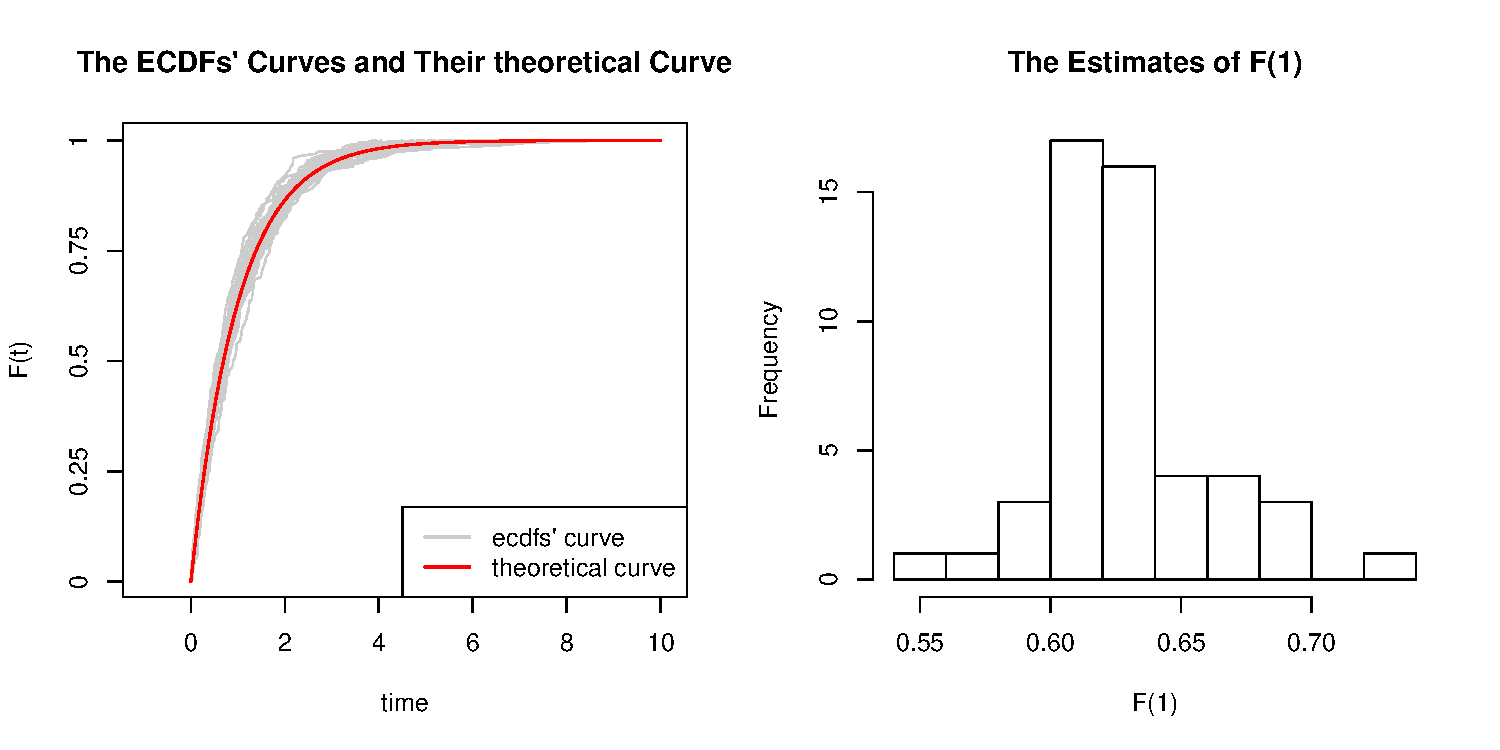
\includegraphics[width = 6 in]{3_10_ab.pdf}
		\end{figure}	
	}
	
 	\item[(c)]{and (d)
		\begin{figure}[h]
			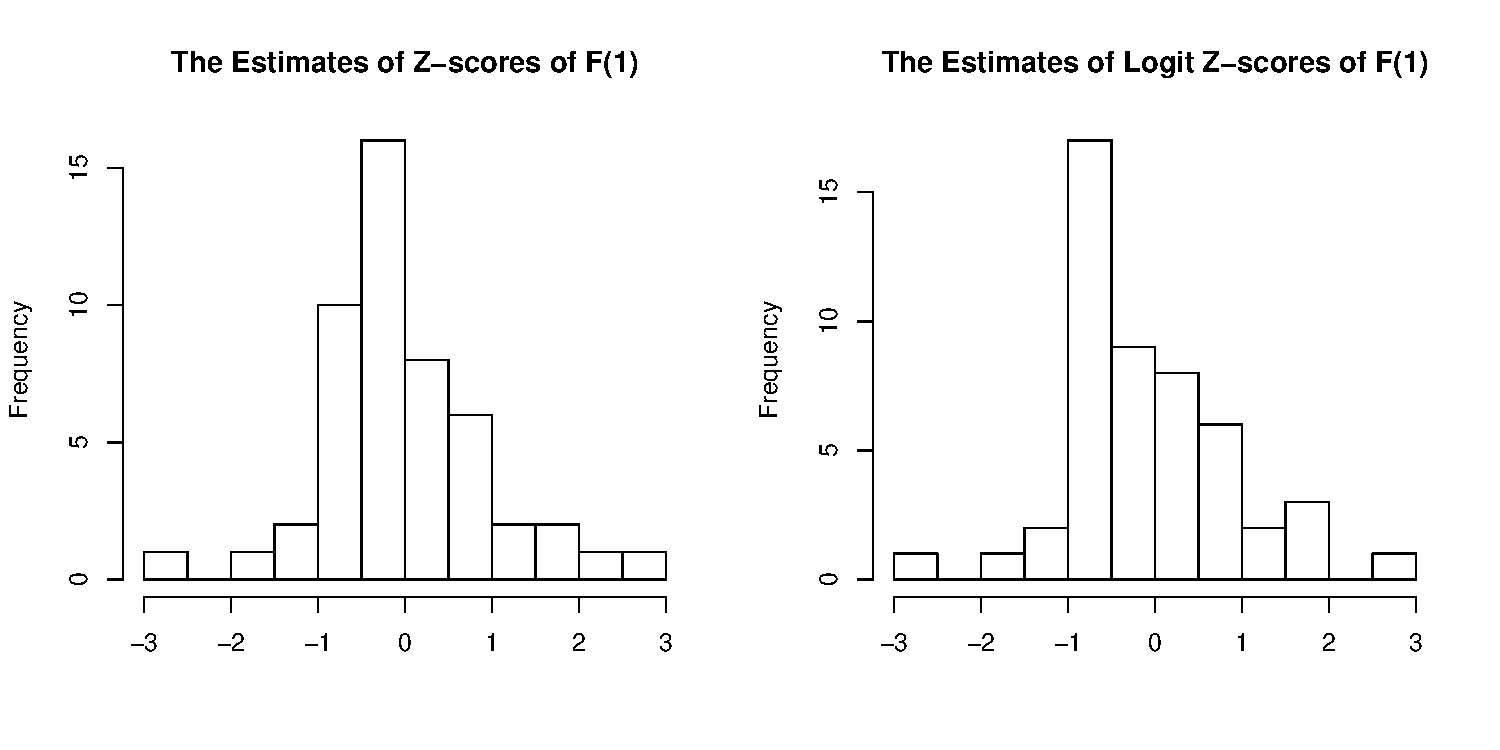
\includegraphics[width = 6 in]{3_10_cd.pdf}
		\end{figure}		
	}
 	\item[(e)]{
		The original estimates of  $Z-$scores of F(1) are more like a normal distribution. 
	}
\end{itemize}


\newpage
%----------------------------------------------------------------------------------------
%	3.14
%----------------------------------------------------------------------------------------
3.14
\begin{align*}
			&	\text{By applying the $\delta-$method: \ \ } Var(g(\widehat{\theta})) = \left( \frac{dg}{d\theta}\right)^2Var(\widehat{\theta}) \\
			&	\text{Let\ \ } g(F) = logit(F) = log(\frac{F}{1-F}) \text{\ \ ,  then\ \ } \frac{dg}{dF}=\frac{1-F}{F}\frac{(1-F)+F}{(1-F)^2} = \frac{1}{F(1-F)}\\
\Rightarrow \ \ \	&	Var(logit(\widehat{F})) = \left( \frac{1}{F(1-F)} \right)^2 Var(\widehat{F})\\
\Rightarrow \ \ \	&	se_{logit(\widehat{F})} = \sqrt{Var(logit(\widehat{F}))} = \frac{se_{\widehat{F}}}{F(1-F)}\\
\Rightarrow \ \ \	&	\widehat{se}_{logit(\widehat{F})} = \frac{\widehat{se}_{\widehat{F}}}{\widehat{F}(1-\widehat{F})}\\
			&	\text{By (3.15), \ \ } Z_{logit(\widehat{F})} = \frac{logit(\widehat{F}) - logit(F)}{se_{logit(\widehat{F})}} \sim N(0, 1)\\
			&	Pr\left( \left|  \frac{logit(\widehat{F}) - logit(F)}{se_{logit(\widehat{F})}} \right| \leq Z_{1-\frac{\alpha}{2}}\right) = 1-\alpha\\
\Rightarrow \ \ \	&	-Z_{1-\frac{\alpha}{2}} \leq \frac{logit(\widehat{F}) - logit(F)}{se_{logit(\widehat{F})}} \leq Z_{1-\frac{\alpha}{2}}\\
\Rightarrow \ \ \	&	logit(F) \in \left[logit(\widehat{F}) - Z_{1-\frac{\alpha}{2}}se_{logit(\widehat{F})}\ \ ,\ \   logit(\widehat{F}) + Z_{1-\frac{\alpha}{2}}se_{logit(\widehat{F})}\right]\\
			&	\text{For\ \ }logit^{-1}(v) = \frac{1}{1+exp(-v)}\ \ , \\
F(t)	\in		&	\left[  \frac{1}{1+exp\left(-(logit(\widehat{F}) - Z_{1-\frac{\alpha}{2}}se_{logit(\widehat{F})})\right)}\ \ ,\ \ \frac{1}{1+exp\left(-(logit(\widehat{F}) + Z_{1-\frac{\alpha}{2}}se_{logit(\widehat{F})})\right)} \right]\\
		=	&	\left[ \frac{1}{1+\frac{1-\widehat{F}}{\widehat{F}}exp\left( Z_{1-\frac{\alpha}{2}} \frac{se_{\widehat{F}}}{F(1-F)} \right)}\ \ , \ \  \frac{1}{1+\frac{1-\widehat{F}}{\widehat{F}}exp\left( -Z_{1-\frac{\alpha}{2}} \frac{se_{\widehat{F}}}{F(1-F)} \right)} \right]\\
		=	&	\left[ \frac{\widehat{F}}{\widehat{F}+(1-\widehat{F})w} \ \ , \ \  \frac{\widehat{F}}{\widehat{F}+(1-\widehat{F})w^{-1}}\right] \ \ \text{\ \ ,where}\ \ w = exp\left( Z_{1-\frac{\alpha}{2}} \frac{se_{\widehat{F}}}{F(1-F)} \right)
\end{align*}
%------------------------------------------------
\end{document}